\chapter{Modification des QoS}
\label{annexe:qos}

\section{Python}

Dans Python, les QoS sont configurés avec des objets \textit{QoSProfile}. Voici un exemple de création d’un publisher avec une fiabilité \textit{Best Effort} (\underline{Source :}\href{https://github.com/PX4/px4_ros_com/blob/e18248db6211350e6a418cb08ae38f64c314a2f4/src/examples/offboard_py/offboard_control.py}{Exemple PX4 Offboard Python})
 :

\begin{lstlisting}[style=commandstyle, caption={Publisher avec QoS personnalisé}]
from rclpy.qos import QoSProfile, QoSReliabilityPolicy
import rclpy
from std_msgs.msg import String

rclpy.init()

node = rclpy.create_node('qos_publisher')

qos_profile = QoSProfile(
    depth=10,
    reliability=QoSReliabilityPolicy.BEST_EFFORT
)

publisher = node.create_publisher(String, 'topic_name', qos_profile)
\end{lstlisting}

\noindent Pour le subscriber :

\begin{lstlisting}[style=commandstyle, caption={Subscriber avec QoS personnalisé}]
from rclpy.qos import QoSProfile, QoSReliabilityPolicy

qos_profile = QoSProfile(
    depth=10,
    reliability=QoSReliabilityPolicy.BEST_EFFORT
)

subscriber = node.create_subscription(
    String,
    'topic_name',
    callback,
    qos_profile
)
\end{lstlisting}

\newpage
\section{Matlab/Simulink}

\subsection{Matlab}

\noindent \underline{Source :} \href{https://fr.mathworks.com/help/ros/ug/manage-quality-of-service-policies-in-ros2.html}{Documentation Matlab}

\begin{lstlisting}[style=commandstyle, caption={Publisher ROS 2 Matlab}]
node = ros2node('matlab_node');
pub = ros2publisher(node, '/topic_name', 'std_msgs/String', ...
    'Depth', 10, 'Reliability', 'besteffort');
\end{lstlisting}

\begin{lstlisting}[style=commandstyle, caption={Subscriber ROS 2 Matlab}]
sub = ros2subscriber(node, '/topic_name', 'std_msgs/String', ...
    'Depth', 10, 'Reliability', 'besteffort', ...
    'Callback', @(msg)disp(msg.data));
\end{lstlisting}

\subsection{Simulink}

Dans Simulink, les blocs ROS Publish et ROS Subscribe peuvent aussi être configurés avec des paramètres QoS :

\begin{itemize}
  \item Double-cliquer sur le bloc \textit{Subscribe} ou \textit{Publish}.
  \item Dans l’onglet \textbf{QoS Settings}, il est possible de modifier les QoS
\end{itemize}

\begin{figure}[H]
    \centering
    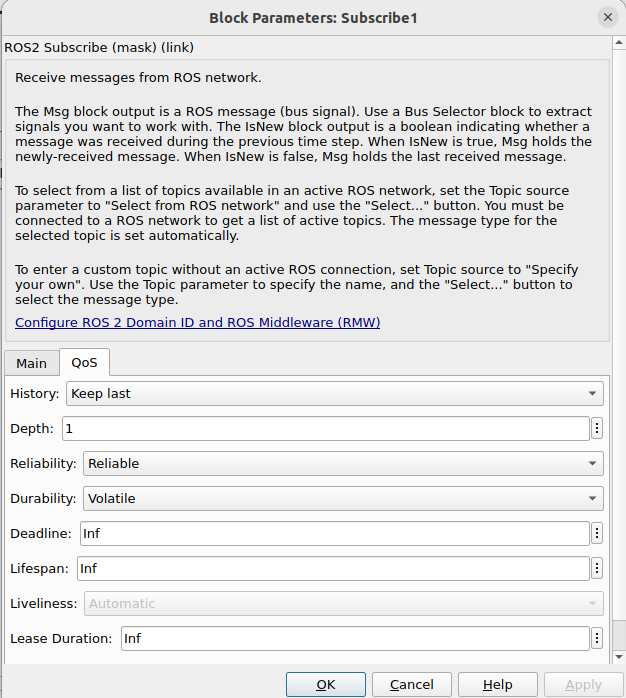
\includegraphics[scale=0.4]{Annexes/pictures/simulink_qos.png}
    \caption{Paramétrage des QoS sur Simulink}
\end{figure}

